\documentclass[11pt]{beamer}  %% versione proiettore
%%\documentclass[11pt,handout]{beamer} %% versione stampa
\usepackage{lucidiJb-2ed}

\usepackage{relsize}

\mode<article>
{
  \usepackage{fullpage}
  \usepackage{hyperref}
}

\mode<presentation>
{
  \setbeamertemplate{background canvas}[vertical shading][bottom=red!10,top=blue!10]
  \usetheme{Ethereum}
  \usefonttheme[onlysmall]{structurebold}
}

\subtitle{Learning Ethereum}
\title{Smart Contracts}
\institute{Universit\`a di Verona, Italy}
\date{January 2020}

\setbeamercovered{invisible}

\def\codesize{\smaller}
\def\<#1>{\codeid{#1}}
\newcommand{\codeid}[1]{\ifmmode{\mbox{\codesize\ttfamily{#1}}}\else{\codesize\ttfamily #1}\fi}

\begin{document}

\begin{frame}
  \titlepage
\end{frame}

\begin{frame}\frametitle{A simple Ponzi scheme}

  \begin{center}
    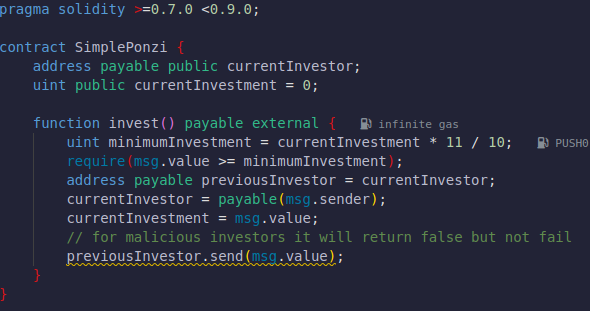
\includegraphics[width=\textwidth,clip=false]{pictures/simple-ponzi.png}
  \end{center}

  \bigskip

  The first investment will be burned to the address \<0x0>.
  
\end{frame}

\begin{frame}\frametitle{Exercise}
  \begin{enumerate}
  \item create an account with MetaMask
  \item charge it from the Ropsten faucet with 1 ETH
  \item write the \<SimplePonzi.sol> contract in Remix
  \item compile the contract in Remix
  \item deploy the contract in Ropsten with Remix
  \item connect to the contract in Ropsten by somebody else
  \item start calling the fallback function with increasing value
    (with Remix of with MetaMask; for the latter, remember to increase
    to gas limit for sending ETH)
  \end{enumerate}

  \bigskip
  You can check the current investment and investor from Remix.

\end{frame}

\begin{frame}\frametitle{A gradual Ponzi scheme}

  \begin{center}
    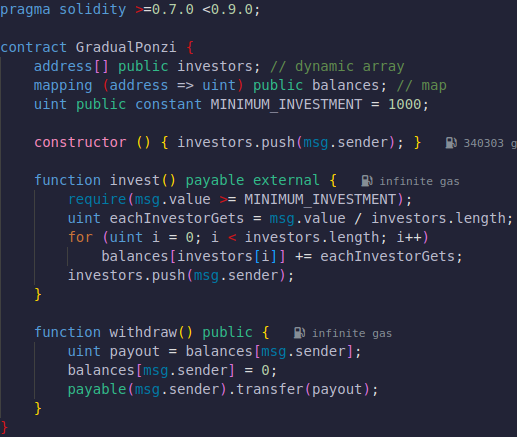
\includegraphics[scale=0.4,clip=false]{pictures/gradual-ponzi.png}
  \end{center}

\end{frame}

\begin{frame}\frametitle{A simple lottery (1)}

  \begin{center}
    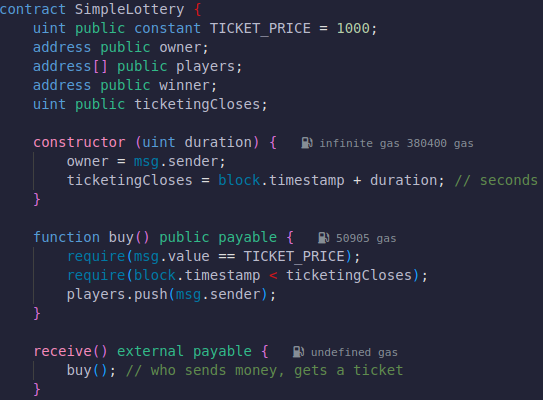
\includegraphics[scale=0.4,clip=false]{pictures/simple-lottery-1.png}
  \end{center}

\end{frame}

\begin{frame}\frametitle{A simple lottery (2)}

  \begin{center}
    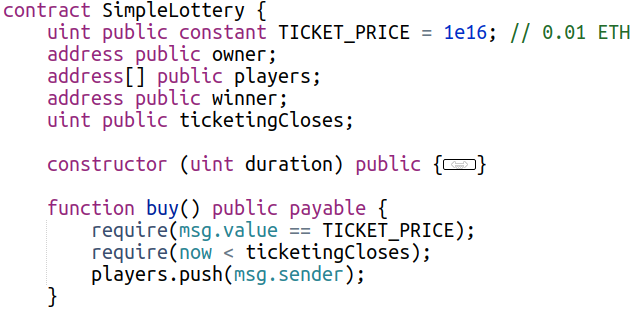
\includegraphics[scale=0.4,clip=false]{pictures/simple-lottery-2.png}
  \end{center}

\end{frame}

\begin{frame}\frametitle{A simple lottery (3)}

  \begin{center}
    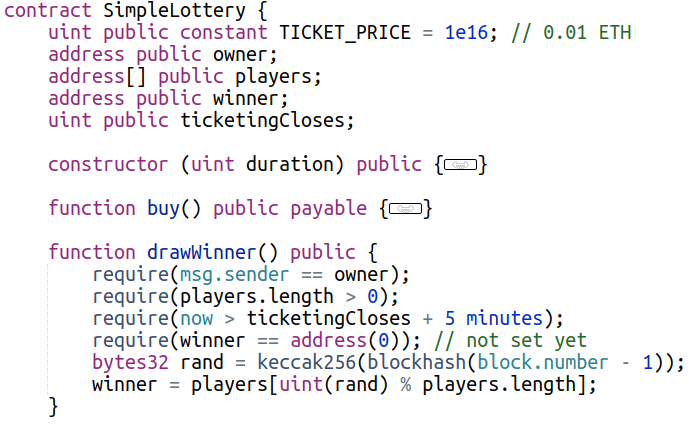
\includegraphics[scale=0.4,clip=false]{pictures/simple-lottery-3.png}
  \end{center}

\end{frame}

\begin{frame}\frametitle{A simple lottery (4)}

  \begin{center}
    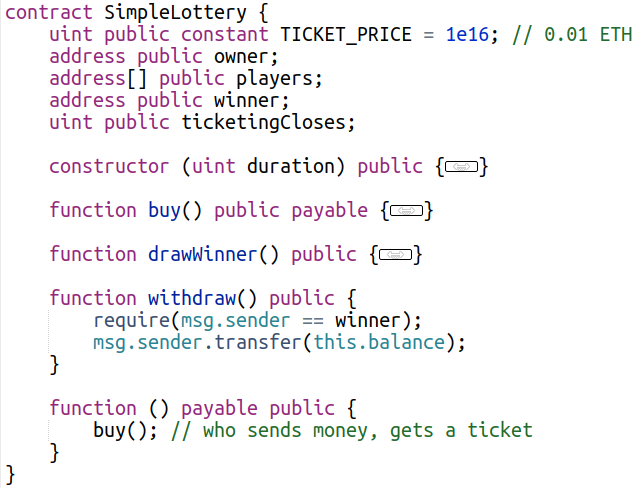
\includegraphics[scale=0.4,clip=false]{pictures/simple-lottery-4.png}
  \end{center}

\end{frame}

\begin{frame}\frametitle{Exercise}
  \begin{enumerate}
  \item create an account with MetaMask
  \item charge it from the Ropsten faucet with 1 ETH
  \item write the \<SimpleLottery.sol> contract in Remix
  \item compile the contract in Remix
  \item deploy the contract in Ropsten with Remix, with 3 minutes for buying tickets
  \item connect to the contract in Ropsten by somebody else
  \item buy some tickets before the 3 minutes expire
    (with Remix of with MetaMask; for the latter, remember to increase
    to gas limit for sending ETH)
  \item the owner of the lottery contract draws the winner
  \item try to withdraw your price (if any!)
  \end{enumerate}

  \bigskip
  You can check the winner from Remix.

\end{frame}

\begin{frame}\frametitle{A simple auction (1)}

  \begin{center}
    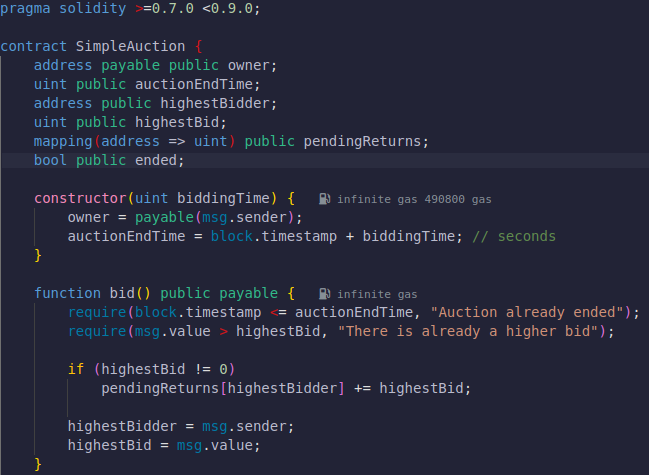
\includegraphics[scale=0.5,clip=false]{pictures/simple-auction-1.png}
  \end{center}

\end{frame}

\begin{frame}\frametitle{A simple auction (2)}

  \begin{center}
    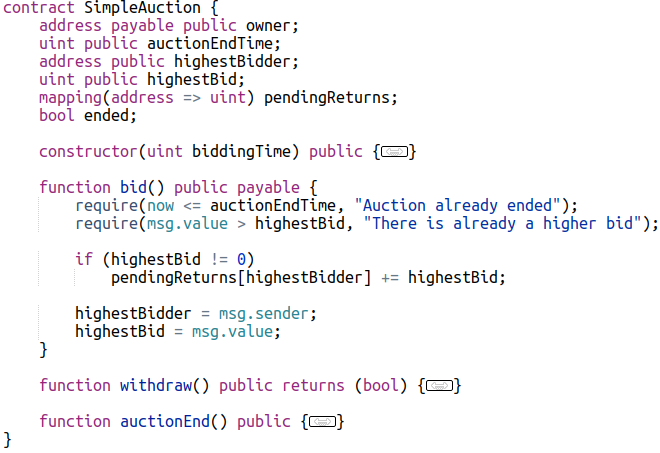
\includegraphics[scale=0.42,clip=false]{pictures/simple-auction-2.png}
  \end{center}

\end{frame}

\begin{frame}\frametitle{A simple auction (3)}

  \begin{center}
    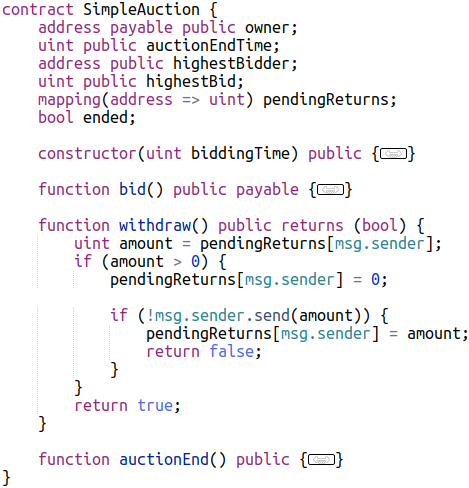
\includegraphics[scale=0.4,clip=false]{pictures/simple-auction-3.png}
  \end{center}

\end{frame}

\begin{frame}\frametitle{A simple auction (4)}

  \begin{center}
    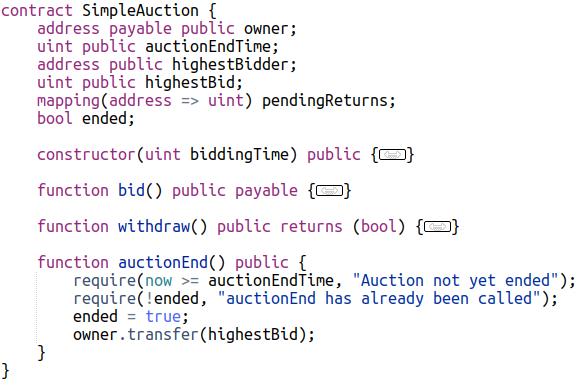
\includegraphics[scale=0.5,clip=false]{pictures/simple-auction-4.png}
  \end{center}

\end{frame}

\begin{frame}\frametitle{Why this complicated withdraw pattern?}

  \begin{center}
    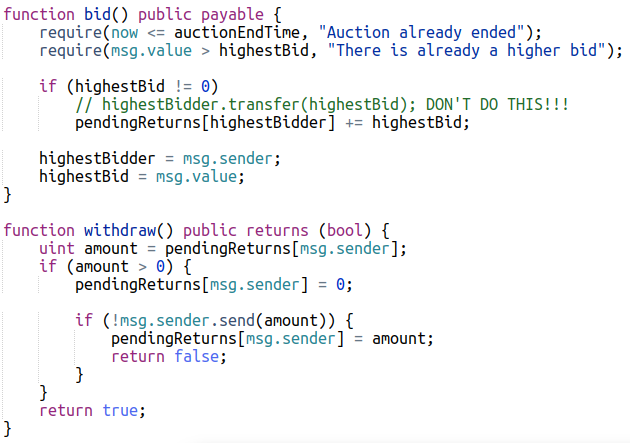
\includegraphics[scale=0.5,clip=false]{pictures/simple-auction-withdraw.png}
  \end{center}

\end{frame}

\begin{frame}\frametitle{Why this complicated withdraw pattern?}

  \begin{greenbox}{\<highestBidder.transfer(highestBid); DON'T DO THIS!!!>}
    The problem with this call (inside function \<bid()>) is that
    a broken or malicious bidder might redefine its own fallback function in
    such a way to consume all gas (for instance):
    \begin{itemize}
    \item all subsequent bidders will get a failure when calling \<bid()>
    \item the broken or malicious contract will never be replaced by another bidder
    \item it will be the winner of the auction, even with a minimal bid!
    \end{itemize}
  \end{greenbox}

\end{frame}

\begin{frame}\frametitle{The re-entrancy nightmare}

  \only<1>{
  \begin{center}
    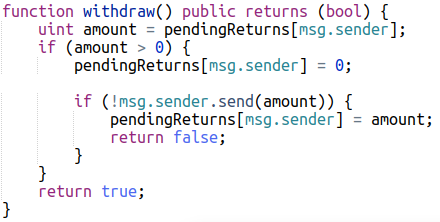
\includegraphics[scale=0.5,clip=false]{pictures/simple-auction-withdraw-only.png}
  \end{center}
  }
  \only<2>{
  \begin{center}
    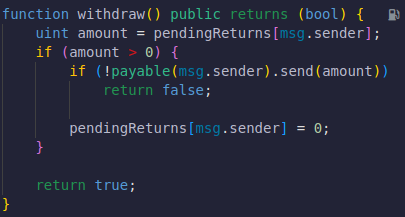
\includegraphics[scale=0.5,clip=false]{pictures/simple-auction-withdraw-only-wrong.png}
  \end{center}
  }

  \only<1>{
    Why this complication of setting \<pendingReturns[msg.sender]=0>
    so early?
  }
    
  \only<2>{
  \begin{greenbox}{Order does matter}
    \begin{itemize}
    \item a malicious bidder might redefine its own fallback function
      in order to call \<withdraw()> back again, as many times as it likes
    \item it will withdraw its \<amount> as many times as it wants, until
      the auction contract is depleted
    \item basically, it runs away with the bids of all bidders
    \end{itemize}
  \end{greenbox}
  }

\end{frame}

\begin{frame}\frametitle{The re-entrancy nightmare}

  \begin{center}
    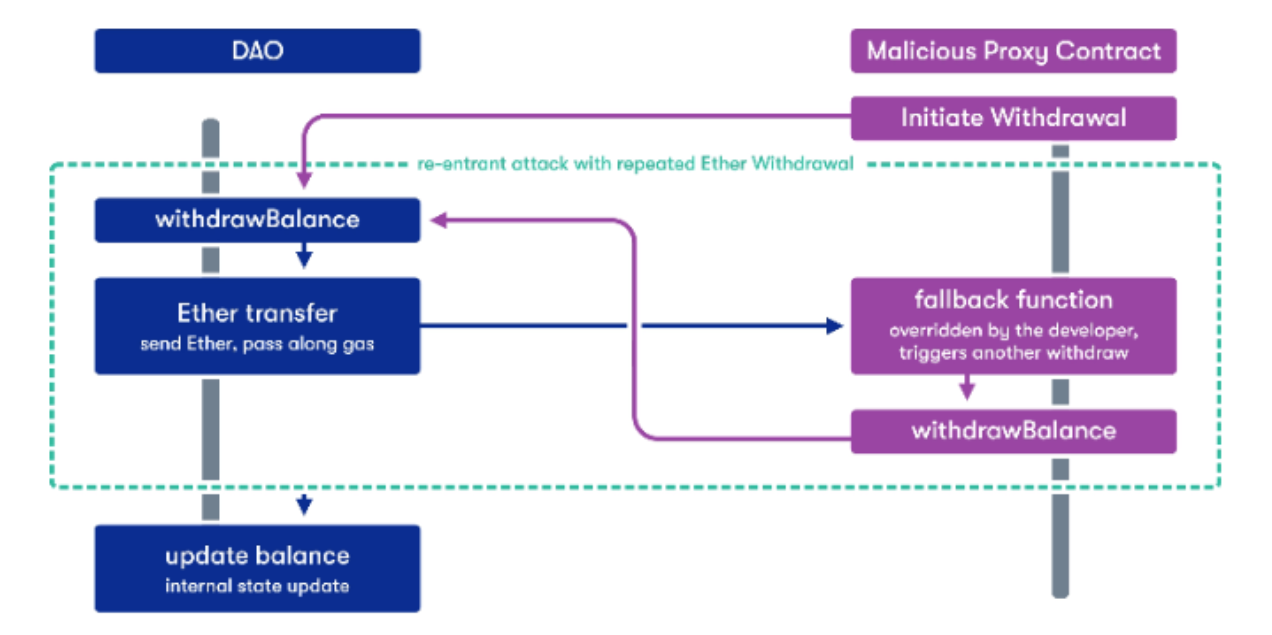
\includegraphics[width=\textwidth,clip=false]{pictures/re-entrancy.png}
  \end{center}

\end{frame}

\begin{frame}\frametitle{The DAO attack (2016)}

  \begin{greenbox}{The most famous re-entrancy exploit}
    \begin{itemize}
    \item the DAO was a contract for autonomous decentralized organizations
    \item the attacker used re-entrancy to steal $50M\$$ equivalent of ETH
    \item the Ethereum team decided to change the consensus rules in order
      to make such transactions illegal and get some of that money back
    \item some node maintainers didn't accept the change and continued
      operating with the old rules, leading to a network fork known as
      Ethereum Classic
    \end{itemize}
  \end{greenbox}

  \begin{center}
    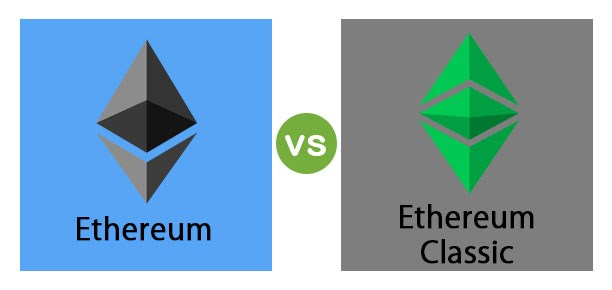
\includegraphics[scale=0.5,clip=false]{pictures/ethereum-vs-ethereum-classic.jpg}
  \end{center}

\end{frame}

\begin{frame}[fragile]\frametitle{Are \<send()> and \<transfer()> safe from re-entrancy?}

  \begin{greenbox}{Currently yes}
    \begin{itemize}
    \item they only forward $2300$ units of gas, not enough for re-entrancy
    \item differently from the low-level \verb!msg.sender.call.value(amount)("")!, that forwards all gas and definitely allows re-entrancy
    \item however:
      \begin{itemize}
      \item gas costs might change in the future, allowing re-entrancy also
        with $2300$ units of gas
      \item the programmer might decide to forward more gas explicitly in order to deal
        with contracts with complex fallback functions
      \item \<send()> and \<transfer()> risk to be deprecated soon\ldots
      \end{itemize}
    \item in conclusion, it's good practice to
      set \<pendingReturns[msg.sender] = 0>
      before sending the money to
      \<msg.sender>, however this is done
    \end{itemize}
  \end{greenbox}

\end{frame}

\end{document}
